
\noindent\begin{minipage}{\textwidth}
    \begin{table}[H]
        \centering
        \caption{Hiperparâmetros e Resultados do Melhor Modelo - vit\_v1\_AB\_opt}
        \vspace{0.2cm}
        \resizebox{\textwidth}{!}{%
            \begin{tabular}{ll | lrrr}
                \hline
                \multicolumn{2}{c|}{\textbf{Hiperparâmetros}} & \multicolumn{4}{c}{\textbf{Métricas por Classe}} \\ \hline
                \textbf{Parâmetro} & \textbf{Valor} & \textbf{Classe} & \textbf{Precisão} & \textbf{Recall} & \textbf{F1-Score} \\ \hline
    Agendador (Patience) & 4 & 31.2 & 0.3867 & 0.4381 & 0.4108 \\ 
Agendador de LR & ReduceLROnPlateau & 31.3 & 0.1889 & 0.0842 & 0.1164 \\ 
Architecture & vit\_b\_16 & 31.4 & 0.2802 & 0.2762 & 0.2782 \\ 
Batch Size & 32 & 32.3 & 0.2944 & 0.3724 & 0.3288 \\ 
Decaimento de Peso (WD) & 0.0592 & 32.4 & 0.0897 & 0.1207 & 0.1029 \\ 
Dropout & 0.0224 & 33.3 & 0.3516 & 0.3316 & 0.3413 \\ 
Função de Perda & CrossEntropyLoss & 41.4 & 0.0545 & 0.0682 & 0.0606 \\ 
Hidden Units & 512 & 41.5 & 0.2083 & 0.2564 & 0.2299 \\ 
Label Smoothing & 0.0815 & 42.4 & 0.3056 & 0.3235 & 0.3143 \\ 
Otimizador & AdamW & 44.4 & 0.2069 & 0.2069 & 0.2069 \\ 
\cline{3-6} 
Taxa de Aprendizado (LR) & 1.92e-04 & \textbf{Média (Macro)} & 0.2403 & 0.2548 & 0.2430 \\ 
Unfreeze Layers & 3 & \textbf{MCC} & \multicolumn{3}{c}{0.1770} \\ 
            \hline
            \end{tabular}%
        }
    \end{table}

    \begin{figure}[H]
        \centering
        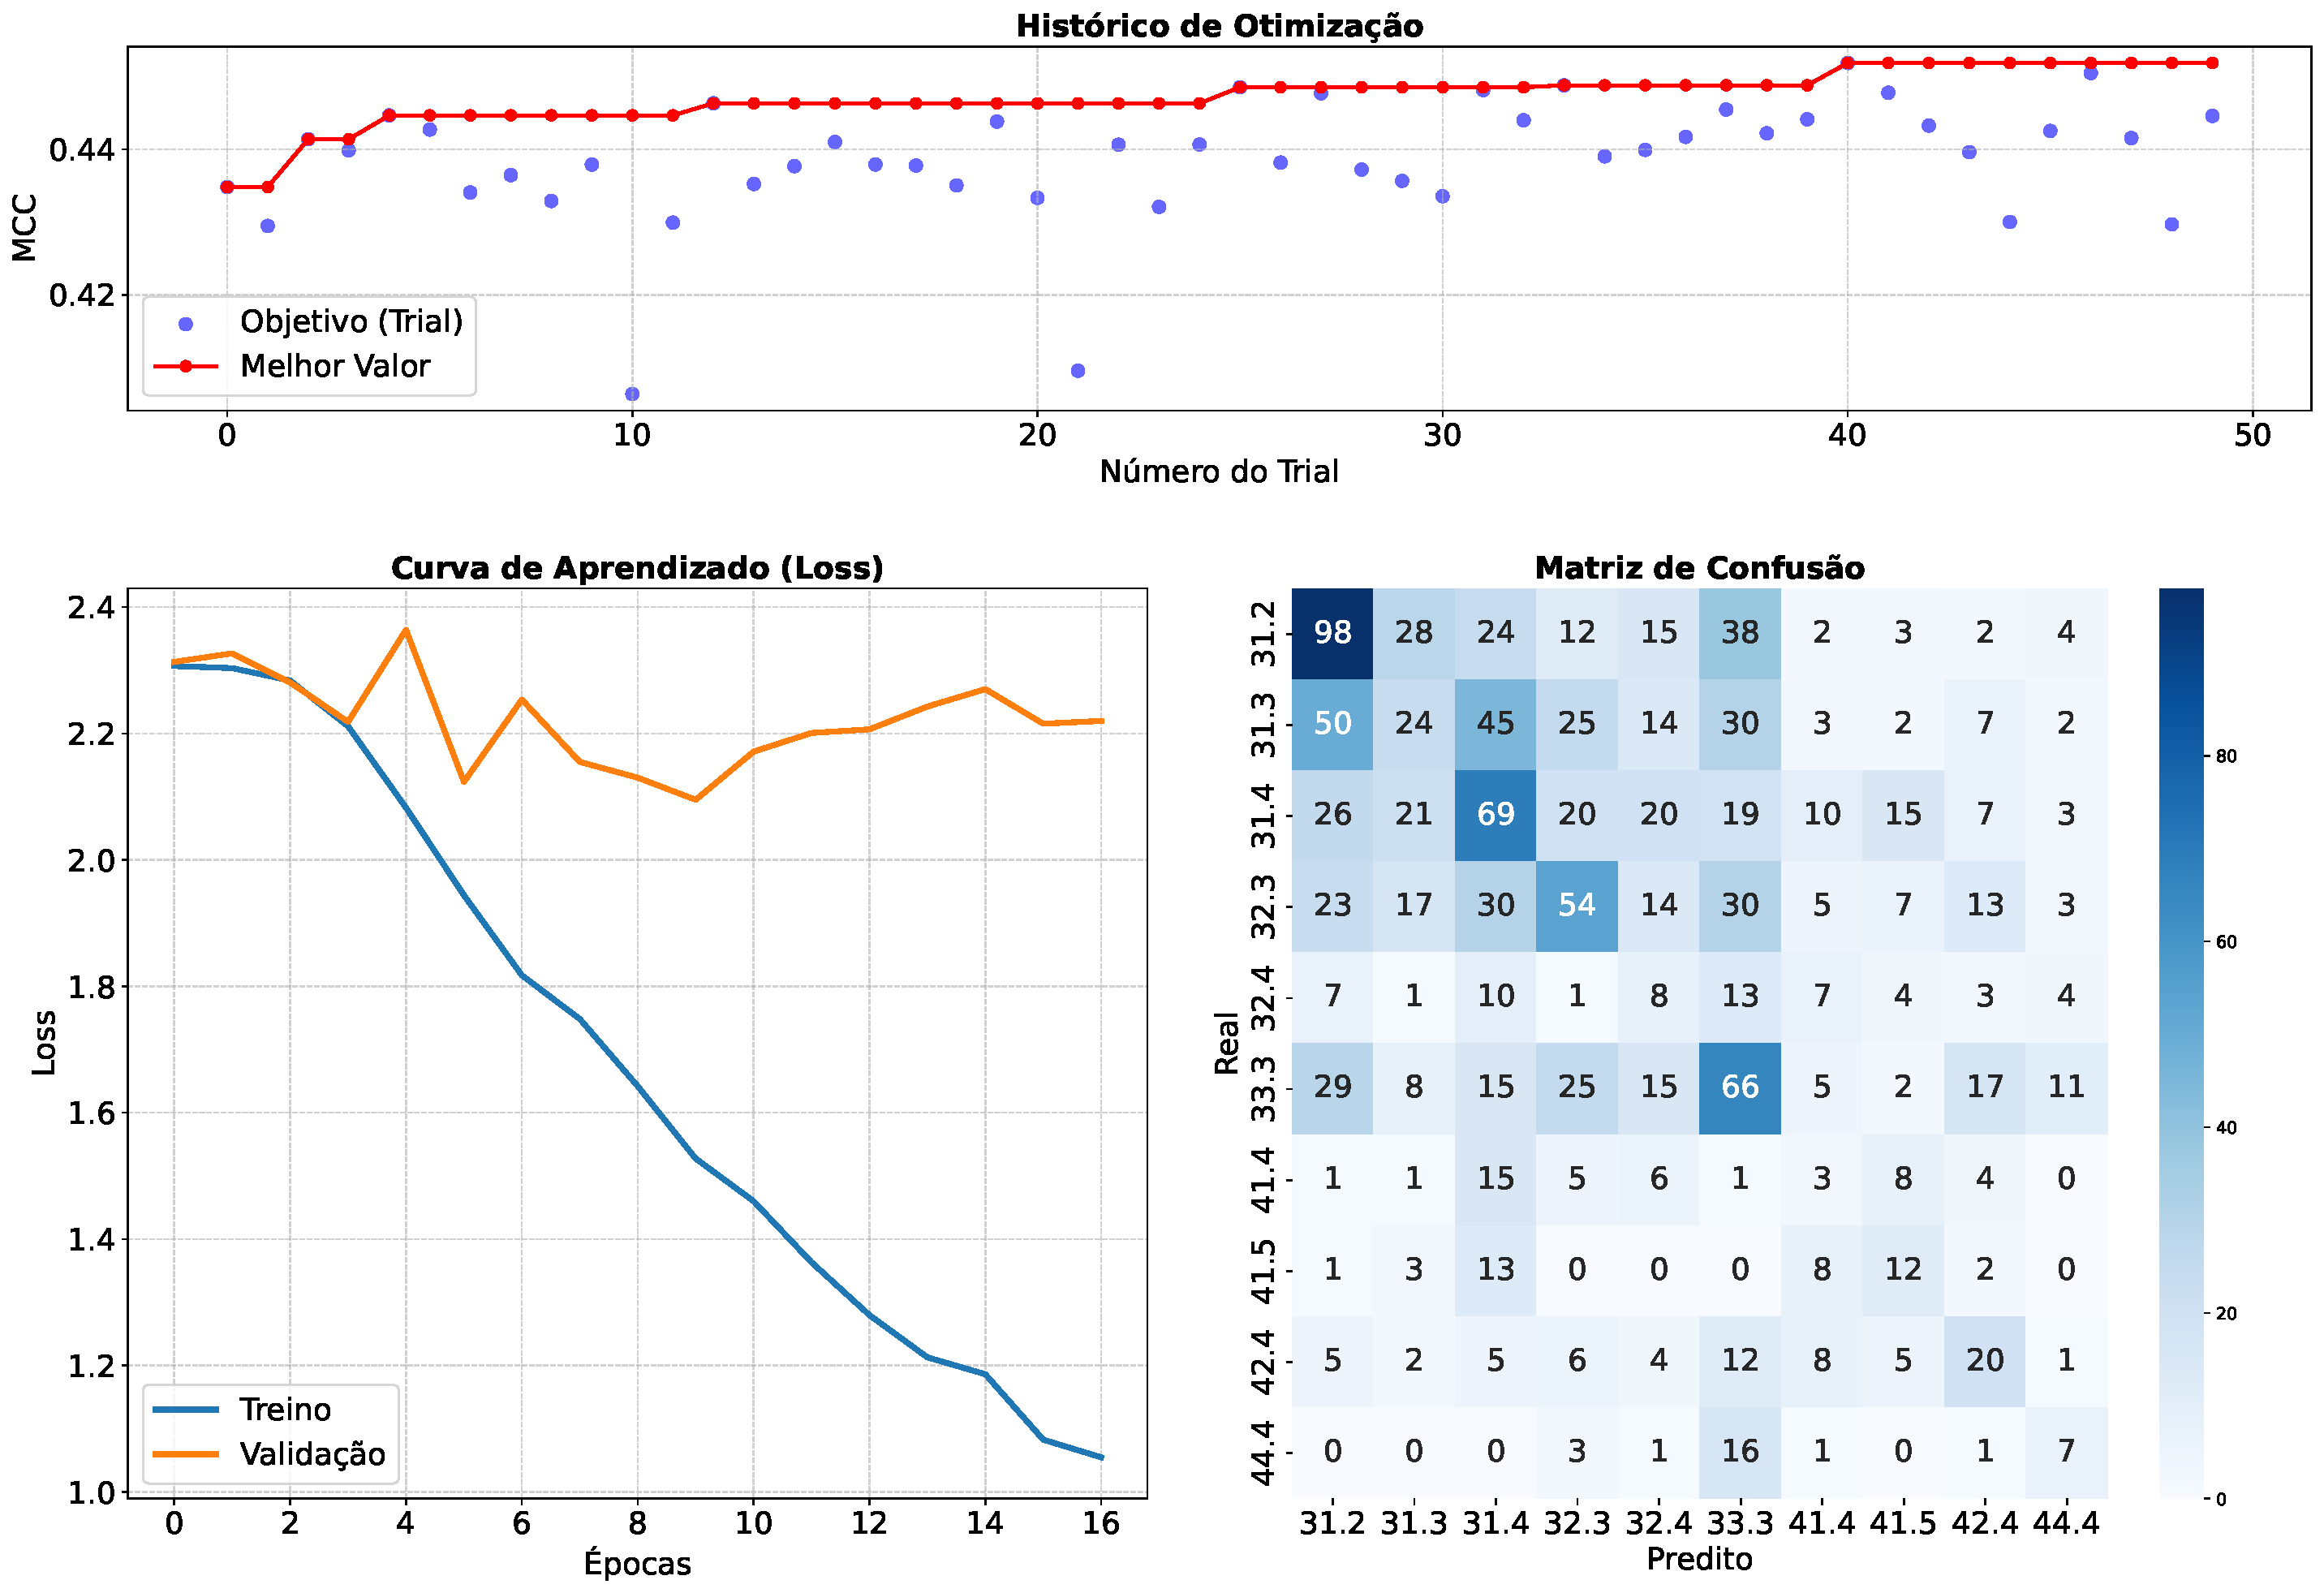
\includegraphics[width=0.85\textwidth]{tex/appendix/experiments/vit_v1_AB_opt/dashboard_consolidado.pdf}
        \caption{Histórico de Otimização, Curvas de Aprendizado e Matriz de Confusão - vit\_v1\_AB\_opt}
    \end{figure}
\end{minipage}
\clearpage
